% Options for packages loaded elsewhere
\PassOptionsToPackage{unicode}{hyperref}
\PassOptionsToPackage{hyphens}{url}
%
\documentclass[
  12pt,
  a4paper]{extarticle}
\title{Analysis 1A --- Tutorial 10}
\author{Christian Jones: University of Bath}
\date{December 2022}

\usepackage{amsmath,amssymb}
\usepackage{lmodern}
\usepackage{iftex}
\ifPDFTeX
  \usepackage[T1]{fontenc}
  \usepackage[utf8]{inputenc}
  \usepackage{textcomp} % provide euro and other symbols
\else % if luatex or xetex
  \usepackage{unicode-math}
  \defaultfontfeatures{Scale=MatchLowercase}
  \defaultfontfeatures[\rmfamily]{Ligatures=TeX,Scale=1}
\fi
% Use upquote if available, for straight quotes in verbatim environments
\IfFileExists{upquote.sty}{\usepackage{upquote}}{}
\IfFileExists{microtype.sty}{% use microtype if available
  \usepackage[]{microtype}
  \UseMicrotypeSet[protrusion]{basicmath} % disable protrusion for tt fonts
}{}
\makeatletter
\@ifundefined{KOMAClassName}{% if non-KOMA class
  \IfFileExists{parskip.sty}{%
    \usepackage{parskip}
  }{% else
    \setlength{\parindent}{0pt}
    \setlength{\parskip}{6pt plus 2pt minus 1pt}}
}{% if KOMA class
  \KOMAoptions{parskip=half}}
\makeatother
\usepackage{xcolor}
\IfFileExists{xurl.sty}{\usepackage{xurl}}{} % add URL line breaks if available
\IfFileExists{bookmark.sty}{\usepackage{bookmark}}{\usepackage{hyperref}}
\hypersetup{
  pdftitle={Analysis 1A --- Tutorial 10},
  pdfauthor={Christian Jones: University of Bath},
  hidelinks,
  pdfcreator={LaTeX via pandoc}}
\urlstyle{same} % disable monospaced font for URLs
\usepackage[margin=2.5cm]{geometry}
\usepackage{longtable,booktabs,array}
\usepackage{calc} % for calculating minipage widths
% Correct order of tables after \paragraph or \subparagraph
\usepackage{etoolbox}
\makeatletter
\patchcmd\longtable{\par}{\if@noskipsec\mbox{}\fi\par}{}{}
\makeatother
% Allow footnotes in longtable head/foot
\IfFileExists{footnotehyper.sty}{\usepackage{footnotehyper}}{\usepackage{footnote}}
\makesavenoteenv{longtable}
\usepackage{graphicx}
\makeatletter
\def\maxwidth{\ifdim\Gin@nat@width>\linewidth\linewidth\else\Gin@nat@width\fi}
\def\maxheight{\ifdim\Gin@nat@height>\textheight\textheight\else\Gin@nat@height\fi}
\makeatother
% Scale images if necessary, so that they will not overflow the page
% margins by default, and it is still possible to overwrite the defaults
% using explicit options in \includegraphics[width, height, ...]{}
\setkeys{Gin}{width=\maxwidth,height=\maxheight,keepaspectratio}
% Set default figure placement to htbp
\makeatletter
\def\fps@figure{htbp}
\makeatother
\setlength{\emergencystretch}{3em} % prevent overfull lines
\providecommand{\tightlist}{%
  \setlength{\itemsep}{0pt}\setlength{\parskip}{0pt}}
\setcounter{secnumdepth}{5}
\newcommand{\BOO}{BOO}
\usepackage {hyperref}
\hypersetup {colorlinks = true, linkcolor = blue, urlcolor = blue}
\usepackage{float}
\ifLuaTeX
  \usepackage{selnolig}  % disable illegal ligatures
\fi

\usepackage{amsthm}
\theoremstyle{plain}
\newtheorem*{theorem*}{Theorem}\newtheorem{theorem}{Theorem}[section]
\theoremstyle{plain}
\newtheorem*{lemma*}{Lemma}\newtheorem{lemma}{Lemma}[section]
\theoremstyle{plain}
\newtheorem*{corollary*}{Corollary}\newtheorem{corollary}{Corollary}[section]
\theoremstyle{plain}
\newtheorem*{proposition*}{Proposition}\newtheorem{proposition}{Proposition}[section]
\theoremstyle{plain}
\newtheorem*{conjecture*}{Conjecture}\newtheorem{conjecture}{Conjecture}[section]
\theoremstyle{definition}
\newtheorem*{definition*}{Definition}\newtheorem{definition}{Definition}[section]
\theoremstyle{definition}
\newtheorem*{example*}{Example}\newtheorem{example}{Example}[section]
\theoremstyle{definition}
\newtheorem*{exercise*}{Exercise}\newtheorem{exercise}{Exercise}[section]
\theoremstyle{remark}
\newtheorem*{remark*}{Remark}
\newtheorem*{solution*}{Solution}
\let\BeginKnitrBlock\begin \let\EndKnitrBlock\end


%\usepackage[english,shorthands=off]{babel}
\usepackage{etoolbox}
\usepackage{spverbatim}
\makeatletter
\@ifpackageloaded{float}{}{\usepackage{float}}
\@ifpackageloaded{adjustbox}{}{\usepackage[Export]{adjustbox}}
\makeatother
\floatplacement{figure}{H}
\newcommand{\scalefactor}{1.2}
\adjustboxset*{min width=\scalefactor\width,max width=\linewidth}
\renewcommand{\familydefault}{phv}
\fontfamily{phv}\selectfont
\renewcommand{\em}{\bf}\renewcommand{\textit}{\textbf}\renewcommand{\emph}{\textbf}\renewcommand{\it}{\bf}\renewcommand{\itshape}{\bf}
\setlength{\parindent}{0.0pt}
\setlength{\parskip}{1.0\baselineskip}
\renewcommand{\baselinestretch}{1.5}\selectfont
\setlength{\mathsurround}{0.2em}
\setlength{\arraycolsep}{0.5cm}\renewcommand{\arraystretch}{1.5}
\addtolength{\jot}{\baselineskip}
\renewcommand{\;}{\,}
\sloppy
\allowdisplaybreaks
\usepackage{amsthm}
\newtheoremstyle{plain}{20pt}{3pt}{}{}{\bfseries}{.\newline\nobreak}{1.0em\nobreak}{}
\newtheoremstyle{definition}{20pt}{3pt}{}{}{\bfseries}{.\newline\nobreak}{1.0em\nobreak}{}
\newtheoremstyle{remark}{20pt}{3pt}{}{}{\bfseries}{.\newline\nobreak}{1.0em\nobreak}{}
\csundef{Proof}
\csundef{endProof}
\newenvironment{Proof}
  {\noindent{\bf Proof.}\hspace*{1em}}% Begin
  {\qed\par}% End
%% When redefining an environment it is vital that it has 
%% the same number of arguments as the original
\renewenvironment{proof}[1][\proofname]
  {\trivlist\item\relax\noindent{\bf {#1}.}\hspace*{1em}}% Begin
  {\qed\endtrivlist}% End

\begin{document}
\maketitle

{
\setcounter{tocdepth}{2}
\tableofcontents
}
\newpage
\pagenumbering{arabic}

\hypertarget{introduction}{%
\section*{Introduction}\label{introduction}}
\addcontentsline{toc}{section}{Introduction}

Here is the material to accompany the 10th Analysis Tutorial on the 12th December. Alternative formats can be downloaded by clicking the download icon at the top of the page. As usual, send comments and corrections to \href{mailto:caj50@bath.ac.uk}{Christian Jones (caj50)}.

\hypertarget{lecture-recap}{%
\section{Lecture Recap}\label{lecture-recap}}

\hypertarget{nested-intervals-theorem}{%
\subsection{Nested Intervals Theorem}\label{nested-intervals-theorem}}

\hypertarget{intervals}{%
\subsubsection{Intervals}\label{intervals}}

Over the last semester, we first studied sequences of numbers, and then we used that theory to study sequences of sums. Now it's time to focus on sequences of sets. In particular, we are going to look at sequences of \emph{intervals}, which are defined as follows:

\BeginKnitrBlock{definition}[Interval]
{\label{def:def1} }Let \(S \subseteq \mathbb{R}\). Then \(S\) is an interval if \(\forall x,y \in S\) with \(x \leq y\), and \(\forall z \in \mathbb{R}\), \(x < z < y\) implies that \(z \in S\).
\EndKnitrBlock{definition}
This definition looks pretty complicated, so we could do with some examples. Firstly, we could construct an interval by taking two real numbers \(a\) and \(b\) with \(a \leq b\), and considering the set \[S_1 = \lbrace s \in \mathbb{R}\; \lvert\; a \leq s \leq b \rbrace.\] Similarly, since all quantities involved in the definition are real numbers, we also find that \(S_2 = \mathbb{R}\) defines an interval. Quite bizarrely, we see via \emph{vacuous reasoning}\footnote{Vacuous reasoning is best summed up with an example. Suppose you were looking into an empty room, and you said that ``everybody in that room was staring at their mobile phone''. As there were no people in the room to begin with, this ends up being a completely true statement.} that \(S_3 = \emptyset\) is also an interval!

Conversely, sets such as \(S_4 = \lbrace 0 \rbrace \cup \lbrace 1 \rbrace\) and \[\mathbb{R}\setminus S_1 = \lbrace s \;\lvert\; s < a \;\; \text{or}\;\; s > b\;\rbrace\] are not intervals.

\hypertarget{the-theorem}{%
\subsubsection{The Theorem!}\label{the-theorem}}

It turns out that if we have a sequence of intervals \((I_n)_{n\in\mathbb{N}}\) which are nested --- so that \(I_{n+1} \subseteq I_n\) for all \(n\in\mathbb{N}\) --- we can construct some major theorems in analysis! To do so; however, requires the following result:

\BeginKnitrBlock{theorem}[Nested Intervals Theorem]
{\label{thm:thm1} }Let \((a_n)_{n\in\mathbb{N}}\) and \((b_n)_{n\in\mathbb{N}}\) be real sequences with \(a_n \leq b_n\) for all \(n\in\mathbb{N}\). Suppose also that for all \(n\in\mathbb{N},\) \([a_{n+1},b_{n+1}] \subseteq [a_{n},b_{n}]\). Then \[\bigcap_{n\in\mathbb{N}}[a_n,b_n] \neq \emptyset.\] Moreover, \[b_n - a_n \to 0 \;\;\text{as $n \to \infty$} \Longrightarrow \exists!\; z \in \bigcap_{n\in\mathbb{N}}[a_n,b_n].\]
\EndKnitrBlock{theorem}
In words, this theorem says that if we have a sequence of closed\footnote{You may not have seen the definitions of open and closed sets before, so these have been added to a section at the end of this document.}, bounded, non-empty, nested intervals of decreasing length, then their intersection is non-empty. If the length of these intervals decreases to zero, then there is a unique\footnote{This is what the symbol \(\exists!\) is referring to --- the exclamation point indicates the unique part of this statement. It is definitely \emph{not} \(\exists! = \exists(\exists-1)\ldots(2)(1).\)} element in this intersection. As you can see, there's a lot of hypotheses for this theorem; Homework Question 1 this week has you going through these hypotheses, and exploring what happens when you remove them.

\hypertarget{sec1}{%
\subsection{Real Functions}\label{sec1}}

\hypertarget{sequential-continuity}{%
\subsubsection{Sequential Continuity}\label{sequential-continuity}}

We've finally reached some of the main results in the course, and certainly ones that will carry you into semester two! Until now, you may have thought of a function being \emph{continuous} if you can draw it without taking your pencil off the page, but we can formalise this idea in the below definition:

\BeginKnitrBlock{definition}[Sequential Continuity]
{\label{def:def2} }Let \(I \subseteq \mathbb{R}\) and \(x_0 \in I\). A function \(f: I \to \mathbb{R}\) is sequentially continuous at \(x_0\) if for all sequences \((x_n)_{n\in\mathbb{N}}\) in \(I\) such that \(x_n \to x_0\) as \(n \to \infty\), we have that \(f(x_n) \to f(x_0)\) as \(n \to \infty\).
\EndKnitrBlock{definition}
This definition looks pretty horrible, but it really amounts to saying that for all convergent sequences in the domain tending to \(x_0\), \[\lim_{n\to\infty}f(x_n) = f\left(\lim_{n\to\infty}x_n\right).\] The main point here is that you need to prove we can swap the limits \textbf{for all} sequences converging to \(x_0.\) You can't just test it for a specific sequence. This is shown graphically in Figure \ref{fig:seqcnt}.

\begin{figure}
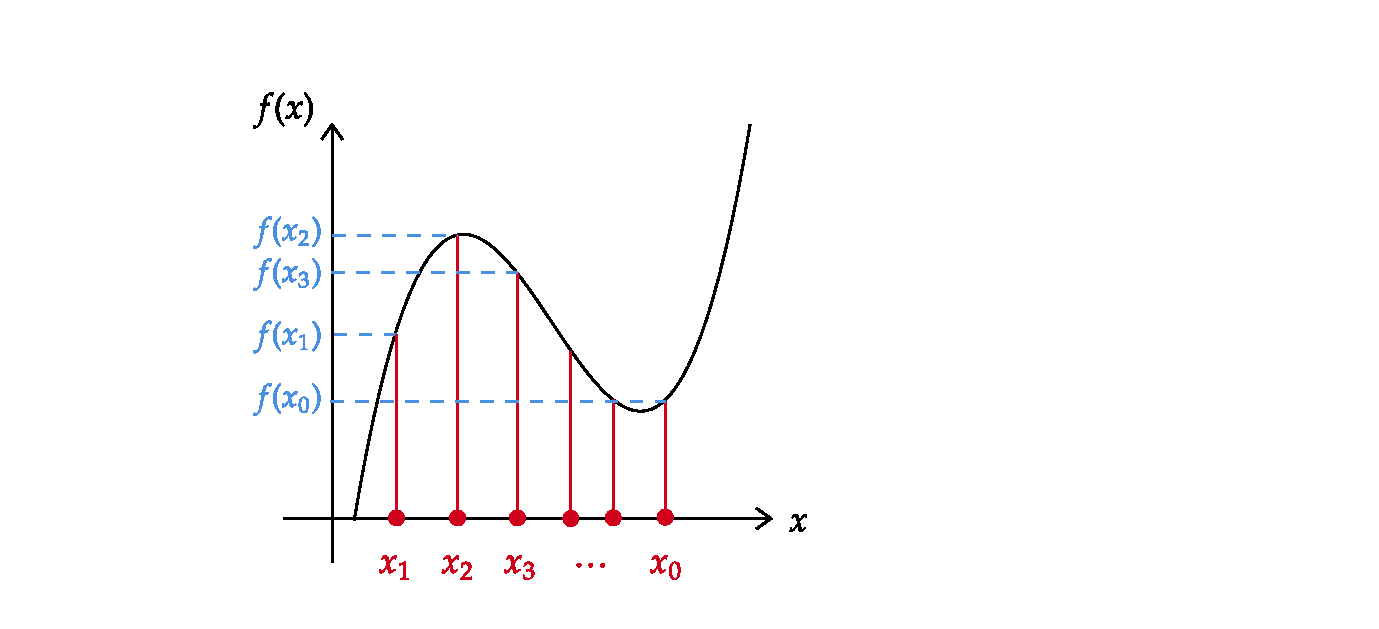
\includegraphics[width=\Width,height=\Height]{Seqcnt} \caption{A diagram showing the idea of sequential continuity. Note that as the values of $x_n$ get closer to the limiting value $x_0$, the corresponding values of $f(x_n)$ get closer to a limiting value $f(x_0)$. This property has to hold for all sequences in the domain converging to $x_0$.}\label{fig:seqcnt}
\end{figure}

Now, having a definition is all well and good, but how do we use it?
\BeginKnitrBlock{example}
{\label{exm:ex1} }Prove that the function \(f: \mathbb{R} \to \mathbb{R}\) given by \[f(x) = x^{27} - 4x^6 + \frac{3}{x^2 +1}\] is sequentially continuous on \(\mathbb{R}\).
\EndKnitrBlock{example}

\BeginKnitrBlock{solution*}
First fix \(x_0 \in \mathbb{R}\), and take \emph{any} sequence \((x_n)_{n\in\mathbb{N}}\) in \(\mathbb{R}\) such that \(x_n \to x_0\) as \(n \to \infty\). Then by the Algebra of Limits
\begin{align*}
f(x_n) &= x_n^{27} - 4x_n^{6} + \frac{3}{x_n^2 +1}\\
&\to x_0^{27} - 4x_0^6 + \frac{3}{x_0^2 + 1}\; \; \text{as $n \to \infty$}\\
& = f(x_0).
\end{align*}
Hence, as the chosen convergent sequence was arbitrary, \(f\) is sequentially continuous at \(x_0\). Since \(x_0\) was arbitrary, \(f\) is sequentially continuous on \(\mathbb{R}\).
\EndKnitrBlock{solution*}

It's also useful to know how to prove a function isn't sequentially continuous at a point. To this end, we conclude this section with a rather interesting example.
\BeginKnitrBlock{example}
{\label{exm:ex2} }Prove that the function \(g: \mathbb{R} \to \mathbb{R}\) given by \[g(x) = \begin{cases}
0 \quad \text{if} \; x \in \mathbb{R}\setminus\mathbb{Q},\\
1 \quad \text{if} \; x \in \mathbb{Q}.
\end{cases}\] is not sequentially continuous anywhere on \(\mathbb{R}\).
\EndKnitrBlock{example}

\BeginKnitrBlock{solution*}
Fix \(x_0 \in \mathbb{R}\). Our aim is to find two sequences \((x_n)_{n\in\mathbb{N}}\) and \((y_n)_{n\in\mathbb{N}}\) converging to \(x_0\), such that \(\left(g(x_n)\right)_{n\in\mathbb{N}}\) and \(\left(g(y_n)\right)_{n\in\mathbb{N}}\) approach different limits. Since both the rational and the irrational numbers are dense in the real numbers, we take \[(x_n)_{n\in\mathbb{N}}\;\; \text{in}\;\; \mathbb{R}\setminus\mathbb{Q} \;\; \text{such that} \;\; x_n \to x_0 \;\; \text{as}\;\; n \to \infty,\] and \[(y_n)_{n\in\mathbb{N}}\;\; \text{in}\;\; \mathbb{Q} \;\; \text{such that} \;\; y_n \to x_0 \;\; \text{as}\;\; n \to \infty.\] Now, note that as \(n \to \infty,\) \[g(x_n) = 0 \to 0, \quad \text{and} \quad g(y_n) = 1 \to 1.\] So, no matter the value of \(g(x_0)\), we have found a sequence --- either \((x_n)_n\) or \((y_n)_n\) --- such that one of \(\left(g(x_n)\right)_n\) or \(\left(g(y_n)\right)_n\) does not tend to \(g(x_0)\). Hence, \(g\) is not sequentially continuous anywhere!
\EndKnitrBlock{solution*}

\hypertarget{intermediate-value-theorem}{%
\subsubsection{Intermediate Value Theorem}\label{intermediate-value-theorem}}

Here's the main reason why we needed the Nested Intervals Theorem!

\BeginKnitrBlock{theorem}[Intermediate Value Theorem (IVT)]
{\label{thm:thm2} }Suppose \(a,b \in \mathbb{R}\) with \(a < b\), and that \(f:[a,b] \to \mathbb{R}\) is sequentially continuous. Then, if \(y \in \mathbb{R}\) is such that either \(f(a) \leq y \leq f(b)\), or \(f(b) \leq y \leq f(a)\), then \(\exists c \in [a,b]\) such that \(f(c) = y\).
\EndKnitrBlock{theorem}
Diagrammatically, we might be in a situation like in Figure \ref{fig:ivt}. Note that there may be more than one \(c\) that fulfills the conclusion of this theorem. Also, the theorem doesn't tell you what this \(c\) is; it only says that a \(c\) must exist.

\begin{figure}
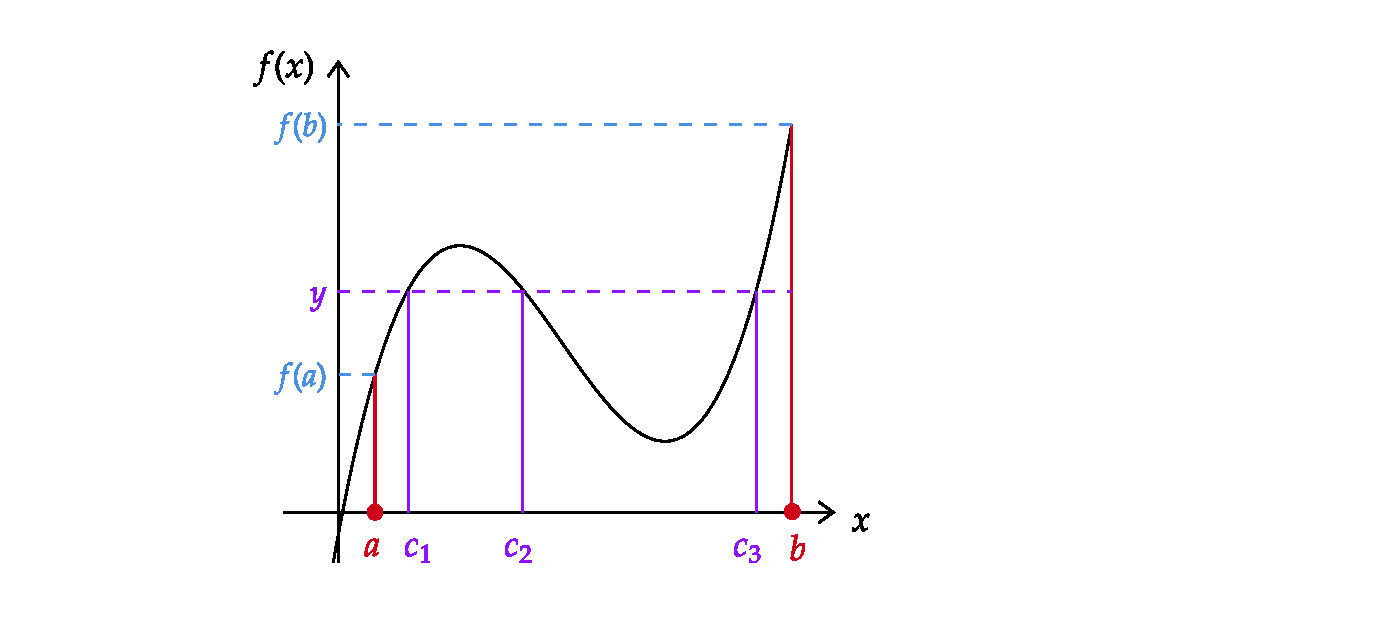
\includegraphics[width=\Width,height=\Height]{ivt} \caption{This function is sequentially continuous on $[a,b]$, and for $y$ as in the diagram, $y$ lies between $f(a)$ and $f(b)$. Hence the IVT applies, and so there exists $c$ in the interval $[a,b]$ such that $f(c)=y$. In this scenario, $c$ can be any one of $c_1,c_2$ or $c_3$.}\label{fig:ivt}
\end{figure}

The IVT is very good for proving existence of square roots (and roots of any degree!), proving that functions have zeros, and proving that at any given point in time, there exists two points on the equator with exactly the same temperature\footnote{On an idealised Earth, anyway.}.

\hypertarget{hints}{%
\section{Hints}\label{hints}}

As per usual, here's where you'll find the problem sheet hints! There's no official hand in this week, but I'll still mark anything handed in by Friday. The questions on this problem sheet are sort of split into two groups. The first two questions are all about theorem hypotheses (and are definitely worth thinking about!) In a way, the third question is about theorem hypotheses too. Question 4 is a more standard example, mainly to check you can perform power series calculations.

\begin{itemize}
\tightlist
\item
  {[}H1.{]} Primarily, the idea is to think of an interval that fits the given description, and explain why the conclusion of the theorem doesn't hold. A word of warning, the empty set \(\emptyset\) is a closed set.
\item
  {[}H2.{]} Pretty much the same idea as H1. The examples required won't necessarily be complicated functions. My best advice is to just play around with this question.
\item
  {[}H3.{]} Check the hypotheses of the Intermediate Value Theorem are satisfied by the given function.
\item
  {[}H4.{]} Look back over the examples from last week, or the first tutorial question from this week.
\end{itemize}

\hypertarget{sets}{%
\section{Sets}\label{sets}}

This week, we've been exposed to a fair few definitions regarding sets, some of which come up a fair bit on the problem sheet. The precise definitions of open and closed sets are non-examinable, but you'll need to be aware of some examples for the exam.

\hypertarget{dense-sets}{%
\subsection{Dense Sets}\label{dense-sets}}

We begin with the concept of a \emph{dense set}.
\BeginKnitrBlock{definition}[Dense Set]
{\label{def:def3} }Let \(S \subseteq \mathbb{R}\). A subset \(T\) of \(S\) is dense in \(S\) if \[\forall s \in S \;\;\text{and}\;\; \forall \epsilon > 0,\; \exists t \in T \;\; \text{such that}\;\; \lvert s - t \rvert < \epsilon.\]
\EndKnitrBlock{definition}
Loosely, this says that we can approximate members of \(S\) pretty well by using members of \(T\) instead. For example, you've seen in lectures that the rational numbers \(\mathbb{Q}\) are dense in the real numbers \(\mathbb{R}\). Equally, we can use this to show that the irrational numbers \(\mathbb{R}\setminus\mathbb{Q}\) are dense in \(\mathbb{R}\) too! A useful proposition arising from this is the following:

\BeginKnitrBlock{proposition}
{\label{prp:prop1} }Let \(T \subseteq S\) be dense in \(S\). Then, for all \(x_0 \in S\), there exists a sequence \((x_n)_n\) in \(T\) such that \((x_n)_n\) converges to \(x_0\) in \(S\).
\EndKnitrBlock{proposition}
This is the property that we used in Example \ref{exm:ex2} of Section \ref{sec1} to generate our convergent sequences! Note that the convergence has to be in \(S\), since \(x_0\) may not be in \(T\) (take for example the sequence \(1, 1.4, 1.41,\ldots\) in \(\mathbb{Q}\) converging to \(\sqrt{2}\).)

\hypertarget{open-and-closed-sets}{%
\subsection{Open and Closed Sets}\label{open-and-closed-sets}}

The next two concepts we discuss here go hand-in-hand, and are quite important for the Nested Intervals Theorem (Theorem \ref{thm:thm1}) and the Intermediate Value Theorem (Theorem \ref{thm:thm2}). We first discuss \emph{open sets}.

\BeginKnitrBlock{definition}[Open Set]
{\label{def:def4} }Let \(S \subseteq \mathbb{R}\). Then \(S\) is open if \[\forall s \in S, \exists \epsilon > 0 \;\; \text{such that} \;\; (s-\epsilon,s+\epsilon) \subseteq S.\]
\EndKnitrBlock{definition}
Some examples here would be useful. Working in \(\mathbb{R}\):

\begin{itemize}
\tightlist
\item
  For any \(a,b \in \mathbb{R}\) with \(a < b\) the interval \((a,b) = \lbrace x \;\lvert\; a < x < b \rbrace\) is open, because for any \(s \in (a,b)\), taking \(\epsilon = \min\left\lbrace s-a, b-s\right\rbrace\), we find that \((s-\epsilon, s + \epsilon) \subseteq (a,b)\).
\item
  Intervals of the form \((a, \infty)\) or \((-\infty, a)\) are open.
\item
  \(\mathbb{R}\) is open.
\item
  The empty set \(\emptyset\) is open (!!)
\end{itemize}

The last of these is vacuously true --- since there's no elements in the empty set, the statement is automatically true. We can use the concept of an open set to define a closed set\footnote{We could instead define `closed-ness' in terms of sequences, but for brevity we defer this to Analysis 2A.}.

\BeginKnitrBlock{definition}[Closed Set]
{\label{def:def5} }Let \(S \subseteq \mathbb{R}\). Then \(S\) is closed if its complement \(\mathbb{R}\setminus S\) is open.
\EndKnitrBlock{definition}
Again, some examples are in order. Working in \(\mathbb{R}\):

\begin{itemize}
\tightlist
\item
  For any \(a,b \in \mathbb{R}\) with \(a < b\) the interval \([a,b] = \lbrace x \;\lvert\; a \leq x \leq b \rbrace\) is closed. This is because \[\mathbb{R}\setminus[a,b] = (-\infty,a)\cup(b,\infty),\] which is a union of open sets, hence open.
\item
  Intervals of the form \([a, \infty)\) or \((-\infty, a]\) are closed.
\item
  \(\mathbb{R}\) is closed.
\item
  The empty set \(\emptyset\) is closed.
\end{itemize}

\hypertarget{warnings}{%
\paragraph*{Warnings!}\label{warnings}}
\addcontentsline{toc}{paragraph}{Warnings!}

These next few words are hardly inventive, but we need to mention it: \textbf{sets are not doors}! If a set is not open, we can't automatically conclude that it is closed (and vice versa). Similarly, sets can be both open and closed simultaneously. We finish on some examples to illustrate this:

For any \(a,b \in \mathbb{R}\) with \(a < b\):

\begin{itemize}
\tightlist
\item
  the interval \((a,b)\) is open, but \emph{not} closed.
\item
  the interval \([a,b]\) is closed, but \emph{not} open.
\item
  the intervals \((a,b]\) and \([a,b)\) are neither open or closed.
\item
  the sets \(\emptyset\) and \(\mathbb{R}\) are both open and closed.
\end{itemize}

\end{document}
